\documentclass{article}
\usepackage{tikz}
\usepackage{geometry}
\usepackage{luatexja}
\usepackage{pgffor}
\usepackage[dvipsnames]{xcolor}
\usepackage{tikzpeople} 
\renewcommand{\kanjifamilydefault}{\gtdefault}
\renewcommand{\familydefault}{\sfdefault}

\newcommand{\docpaperwidth}{60mm}
\newcommand{\docpaperheight}{30mm}
\geometry{
  papersize={\docpaperwidth,\docpaperheight},
  margin=0cm,
  ignoreall=true
}

\setlength{\parindent}{0cm}
\usetikzlibrary{calc}
\usetikzlibrary{shadings}

\begin{document}
  \center
  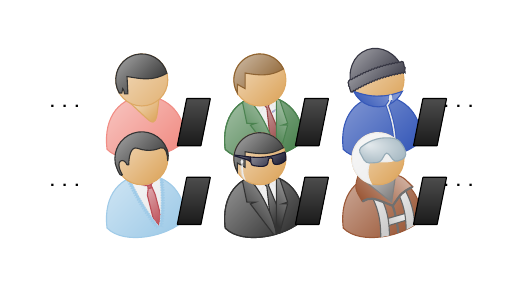
\begin{tikzpicture}
    \path [use as bounding box]
      (-15mm, -10mm) rectangle (45mm, 20mm);
 
    \newcommand{\smartp}[1]{[rounded corners=0.05mm, xslant=0.2]
      (0, 0) rectangle (3mm * #1, 6mm * #1)}

    \newcommand{\aperson}[4]{
      \node[
        #4,
        minimum size=1cm * #1,
        font=\tiny] at (#2, #3) {};
      \path[draw,
        fill,
        bottom color=black!90,
        top color=black!70,
        xshift= #2 - 6mm * #1 + 1cm * #1,
        yshift= #3 - 8mm * #1 + 3mm * #1] \smartp{#1};
    }
    \node at (-1cm, 1cm) {\ldots};
    \aperson{1}{0cm}{1cm}{nurse}
    \aperson{1}{1.5cm}{1cm}{businessman}
    \aperson{1}{3cm}{1cm}{criminal}
    \node at (4cm, 1cm) {\ldots};
    \node at (-1cm, 0cm) {\ldots};
    \aperson{1}{0cm}{0cm}{dave}
    \aperson{1}{1.5cm}{0cm}{maninblack}
    \aperson{1}{3cm}{0cm}{pilot}
    \node at (4cm, 0cm) {\ldots};

  \end{tikzpicture}
\end{document}

